\clearpage
\section{Software Implementation Overview}\label{overview}

\begin{figure}[htbp]
    \centering
    \def\svgwidth{\textwidth} \small
    \input{gfx/diagrams/overview.pdf_tex}
    \caption{Schematic overview of the information flow from the hardware to the reprojection map}
    \label{fig:overview}
\end{figure}

\Cref{fig:overview} shows the flow of information after the raw data is gathered from the hardware setup described in \cref{implementation-platform}: The \texttt{/omniradar\_node} rosnode (\cref{ros-node}) uses \texttt{libomniradar} (\cref{c-bindings-and-library}) to read in the raw data from the radar sensor. The rosmessages transmitted from the node are then stored in a \texttt{rosbag}, which is copied over the network to the machine running the Matlab implementation. In Matlab, the data is preprocessed (\cref{data-preprocessing}), Doppler speeds are estimated (\cref{doppler-estimation-with-the-peak-gradient-algorithm}) and finally the radar reprojection map is constructed (\cref{reprojection-mapping}).

\section{Driver}\label{driver}

\subsection{Omniradar ROS driver}\label{omniradar-ros-driver}

The Omniradar RIC60A comes with a precompiled Matlab MEX driver library.
This works well in a Windows OS on x86-based computers with a Matlab
installation. An early goal was to have the robot carry the radar module
around wireless. One option would have been to mount a Windows laptop on
the Kobuki. However, Omniradar was kind enough to provide the author
with the driver sources under an NDA agreement. This allowed recompiling
the MEX driver for Linux systems. There were some issues with FTDI's
D2XX serial communication library that had to be fixed for Linux
systems. One challenge with the D2XX driver was that Ubuntu
automatically loads the regular FTDI serial IO driver,
\texttt{ftdi\_sio}. This was be solved by unbinding the driver using a
set of udev rules \footnote{\url{https://stackoverflow.com/questions/44529376}}. Another
issue was that due to a bug in the D2XX implementation, the Omniradar
driver would freeze when more than \SI{2}{MB} of data (equivalent to a \SI{20}{ms}
FMCW chirp) were requested. After a lot of debugging, this could be
solved by never requesting a bigger amount of data than was already
available in the D2XX buffer.

\subsubsection{C++ bindings and library}\label{c-bindings-and-library}

Since Matlab does not run on Arm arch processors such as the Odroid on
the Kobuki robot, a new set of platform-independent C++ bindings was
added to the driver. The C++ bindings serve the same purpose as the
Matlab bindings.

To include the library, some files need to be installed or pointed to by
the binary that needs to use it.

\begin{table}[h]
    \centering
    \rowcolors{1}{}{ColorAlternatedRow}
    \begin{tabularx}{\textwidth}
    {%
      >{\setlength{\hsize}{.25\hsize}\raggedright\arraybackslash}X%
      >{\setlength{\hsize}{.325\hsize}\raggedright\arraybackslash}X%
      >{\setlength{\hsize}{.425\hsize}}X%
    }
    \hiderowcolors
    \toprule
        File &
        Default install destination &
        Purpose \\
    \midrule
    \endhead
    \showrowcolors
        omniradar.h &
        /usr/local/include &
        Library header file \\
        
        libomniradar.so &
        /usr/local/lib &
        Dynamically linked shared object \\
        
        51-omniradar.rules, 52-omniradar.rules &
        /etc/udev/rules.d &
        Udev rules to unbind ftdi\_sio \\
    \bottomrule
    \end{tabularx}
    \caption{File installation destinations of libomniradar}
    \label{tab:files}
\end{table}

If the driver source is available, installing the files can be
accomplished from the source directory with

\begin{Shaded}
\begin{Highlighting}[]
\FunctionTok{mkdir}\NormalTok{ build }\KeywordTok{\&\&} \BuiltInTok{cd}\NormalTok{ build}
\FunctionTok{cmake}\NormalTok{ -DCPP_BINDINGS=ON -DMATLAB_BINDINGS=OFF ..}
\FunctionTok{make}
\FunctionTok{sudo}\NormalTok{ make install}
\end{Highlighting}
\end{Shaded}

The driver can then be included in an application. Note that since it is
dynamically linked, the \texttt{ftd2xx}, \texttt{pthread} and
\texttt{dl} libraries dependencies also need to be linked. In a Catkin
\footnote{Catkin is the CMake-based ROS build system} CMakeLists.txt
this would look like

\begin{Shaded}
\begin{Highlighting}[]
\KeywordTok{target_link_libraries}\NormalTok{(}
  \VariableTok{\$\{PROJECT_NAME\}}\NormalTok{_node}
\NormalTok{  omniradar}
\NormalTok{  ftd2xx}
\NormalTok{  pthread}
\NormalTok{  dl}
  \VariableTok{\$\{catkin_LIBRARIES\}}
\NormalTok{)}
\end{Highlighting}
\end{Shaded}

The C++ library offers the same functions as Omniradar's Matlab driver,
with two differences. The optional device index number is 0-based
instead of 1-based and the \texttt{AcquireEcho} functions return (a shared pointer
to) packed data instead of unpacked data for performance reasons. With
the

\begin{Shaded}
\begin{Highlighting}[]
\AttributeTok{static} \BuiltInTok{std::}\NormalTok{shared_ptr< }\BuiltInTok{std::}\NormalTok{vector< }\BuiltInTok{std::}\NormalTok{vector< }\DataTypeTok{uint8_t}\NormalTok{ > > >}\\
\NormalTok{    demultiplex(}\BuiltInTok{std::}\NormalTok{vector<}\DataTypeTok{uint32_t}\NormalTok{> \&packed_data);}
\end{Highlighting}
\end{Shaded}

function, the library offers an easy way to demultiplex the packed data
array into a (shared pointer to a) vector of four vectors - one for each
echo signal of the I/Q channel of left and right receiving antenna.

Useage is simple as the driver follows the RAII principle. Allocation of
an object of type \texttt{Omniradar} causes the library to fully
initialize the RIC60A RDK. After that, the configuration string and the
VCO tuning curve should be set. Omniradar provides some Matlab example
code that measures the sensor's VCO tuning curve. The easiest way to
bring this tuning curve into the C++ domain is to
print\footnote{`['A' 10 'B']` is a quick way to print a newline character between `A` and `B`}
it as C style array, e.g.~with

\begin{Shaded}
\begin{Highlighting}[]
\NormalTok{[ }\StringTok{'#pragma once'} \FloatTok{10} \StringTok{'std::vector<double>'} \FloatTok{10} \KeywordTok{...}\\
\NormalTok{    }\StringTok{'vco_tune \{'}\NormalTok{, sprintf(}\StringTok{'\%.100g, '}\NormalTok{, VCOtune), }\StringTok{'\};'}\NormalTok{ ]}
\end{Highlighting}
\end{Shaded}

and then saving the resulting string as \texttt{vco\_tune.h} include
file.

This setup allowed the development of a ROS node that handles
communication with the radar module on the Linux/Arm based Kobuki robot.

The files comprising \texttt{libomniradar} are publicly available at \url{https://github.com/lalten/libomniradar}.

\subsection{ROS node}\label{ros-node}
A new \texttt{omniradar} ROS package was developed to support the use of
the Omniradar sensor within the ROS environment. A set of
\texttt{roslaunch} launchfiles comes with the package that support the
startup of the Kobuki robot in teleoperation mode, optionally together
with lidar-based Cartographer slam, AMCL localization and an Astra
Orbbec RGBD camera. A simple version to start the only the node to get
radar data would be:

\begin{Shaded}
\begin{Highlighting}[]
\NormalTok{<launch>}\\
\NormalTok{  <node }\AttributeTok{pkg=} \StringTok{"omniradar"} \AttributeTok{type=} \StringTok{"omniradar_node"} \AttributeTok{name=}\StringTok{"omniradar_node"}\\
\NormalTok{    }\AttributeTok{output=}\StringTok{"screen"}\NormalTok{>}\\
\NormalTok{    <param }\AttributeTok{name=}\StringTok{"n_sweeps"} \AttributeTok{value=}"1"\NormalTok{ />}\\
\NormalTok{    <param }\AttributeTok{name=}\StringTok{"t_sweep"}  \AttributeTok{value=}"5"\NormalTok{ />}\\
\NormalTok{  </node>}\\
\NormalTok{</launch>}
\end{Highlighting}
\end{Shaded}

The node sends out the ROS topic \texttt{/omniradar\_node/radar\_raw} of
the custom \texttt{RadarEcho} type, which is defined in RadarEcho.msg as

\begin{Shaded}
\begin{Highlighting}[]
\DataTypeTok{Header} header
\DataTypeTok{string} ric_config
\DataTypeTok{uint8} n_sweeps
\DataTypeTok{float64} t_sweep
\DataTypeTok{uint32[]} packed_echo
\end{Highlighting}
\end{Shaded}


Early versions of the driver unpacked the radar echo bitstream inside
the node and were able to use standard ROS message types like the
\texttt{std\_msgs/ByteMultiArray} message. However, sending out the
packed bitstream proved to be much more efficient in terms of chirp
efficiency \(\eta\). The custom message type also allows to send out the
configuration (RIC configuration string, number and length of FMCW
sweeps) that was used to attain the message's echo. The message's
timestamp and sequential ID is contained in the regular
\texttt{std\_msgs/Header}.

\begin{figure}[htbp]
    \centering
    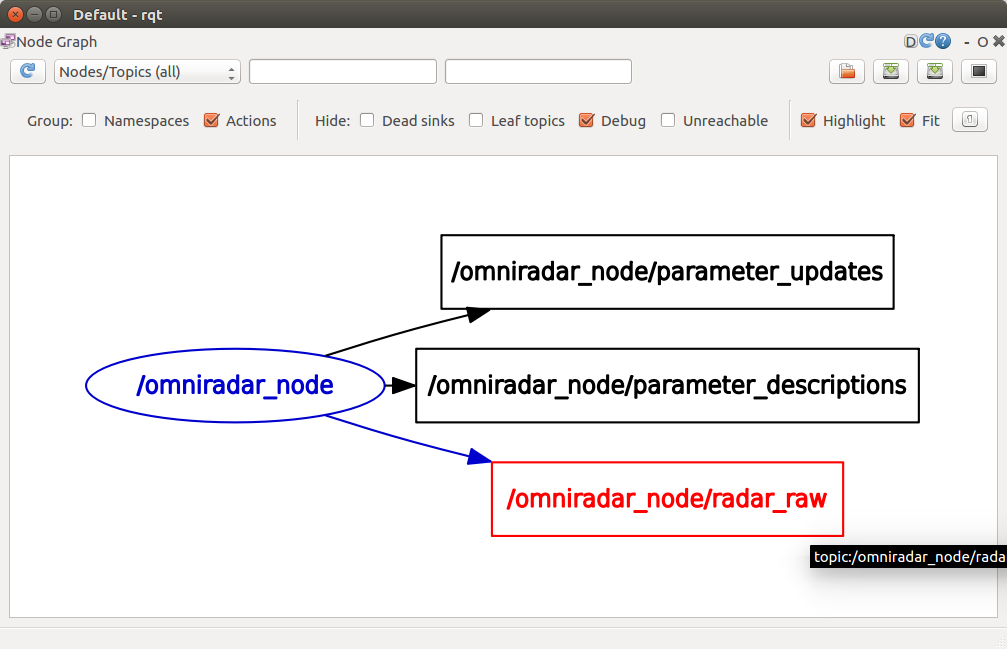
\includegraphics[max height=10cm,max width=10cm]{screenshots/nodegraph}
    \caption{Omniradar rosnode node graph with leaf topics}
    \label{fig:nodegraph}
\end{figure}

While parameters from the ROS parameter server (as configured in the
launch) are respected, the node also offers a dynamic reconfigure server
to change RIC configuration string, number of sweeps and length of sweep
on the fly without the need to restart the node (see \cref{fig:dynreconf}).

\begin{figure}[htbp]
    \centering
    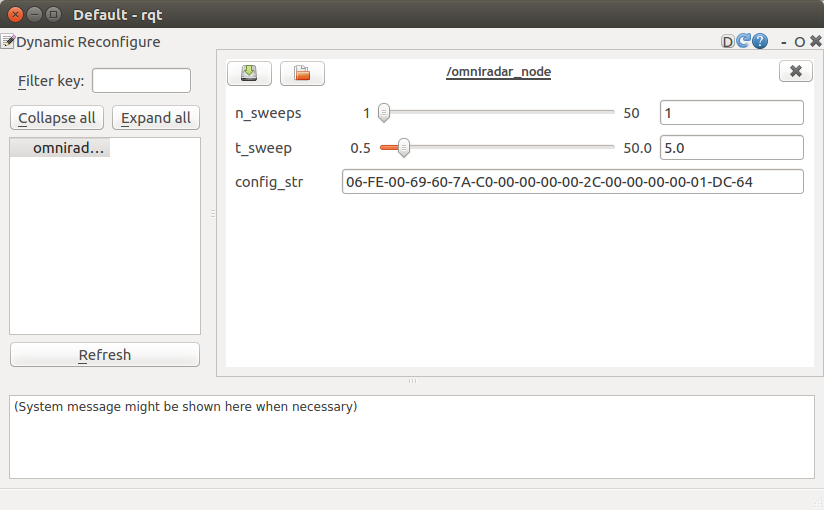
\includegraphics[max height=10cm,max width=10cm]{screenshots/dynreconf}
    \caption{Dynamic reconfigure options for the Omniradar rosnode}
    \label{fig:dynreconf}
\end{figure}

The core of the node is a while loop that continuously triggers radar
echo acquisition and copies the result into a new
\texttt{omniradar::RadarEcho} message. The radar sensor update rate
could be increased by offloading the message assembly and data copying
into a C++11 lambda thread that is immediately detached.

\begin{samepage}
\begin{Shaded}
\begin{Highlighting}[]
\BuiltInTok{std::}\NormalTok{lock_guard<}\BuiltInTok{std::}\NormalTok{mutex> lock_rdk(mtx_rdk);}
\KeywordTok{auto}\NormalTok{ t_echo = ros::Time::now();}
\KeywordTok{auto}\NormalTok{ p_echo = rdk->AcquireEcho(msg.n_sweeps);}

\BuiltInTok{std::}\NormalTok{thread t (}
\NormalTok{    [=] ()}
\NormalTok{    \{}
        \BuiltInTok{std::}\NormalTok{lock_guard<}\BuiltInTok{std::}\NormalTok{mutex> lock_msg(mtx_msg);}
\NormalTok{        msg.header.stamp = t_echo;}
\NormalTok{        msg.packed_echo.resize(p_echo->size());}
        \BuiltInTok{std::}\NormalTok{copy(p_echo->begin(), p_echo->end(), msg.packed_echo.begin());}
\NormalTok{        pub.publish(msg);}
\NormalTok{        msg.header.seq++;}
\NormalTok{    \}}
\NormalTok{);}
\NormalTok{t.detach();}
\end{Highlighting}
\end{Shaded}
\end{samepage}

The multithreading approach lets the node use between \SI{100}{\%} and \SI{140}{\%}
CPU (observed with \texttt{htop}).

The rospackage providing the omniradar rosnode is available at \url{https://github.com/lalten/omniradar}.

\subsection{Matlab interface}\label{matlab}

Matlab (release R2017a) was chosen as implementation platform and language because it allows quick prototyping, provides relatively easy visualization, and, with the Robotics Toolbox, supports many ROS features.

It is necessary to install custom message support with the roboticsAddon\footnote{\url{https://www.mathworks.com/help/robotics/ref/roboticsaddons.html}} and to generate\footnote{\url{https://www.mathworks.com/help/robotics/ug/create-custom-messages-from-ros-package.html}} some files to read in rosbags with the custom \texttt{RadarEcho} type messages.

\section{Data Preprocessing}\label{data-preprocessing}

\subsection{Rosbag to Matlab}\label{rosbag-to-matlab}

Before a target's radar echo can make its way to the map, it passes several stages. In this proof of concept implementation, the map building is done offline, so all data coming out of the omniradar ROS node is recorded in a \texttt{rosbag} for later analysis. This is a good solution because it (1) allows working even without access to hardware, (2) allows quick iteration and prototyping with scripted languages such as Matlab, which are not capable of receiving at real-time speeds, and (3) allows replaying any situation in which an algorithm fails, so that it can be can be tested and improved until the situation can be handled.

The rosbags can be replayed with \texttt{rosbag play} and received in a subscribing \texttt{rosnode} in Matlab. However the replay speed needed to be adjusted to around \SI{10}{\%}, or Matlab will not be able to keep up and will lose some messages. This also the reason why a live system where Ros messages are sent via network to a computer running Matlab is not feasible. A better solution is to read the rosbag files directly into Matlab, using its \texttt{readMessages(bag,rows)}\footnote{\url{https://www.mathworks.com/help/robotics/ref/readmessages.html}}. The system quickly runs into memory problems when reading even a moderately sized bag (e.g. \SI{400}{MB}) at once, because the Java heap space is limited by default. It is not only safer (no \texttt{java.lang.OutOfMemoryError: GC overhead limit exceeded} crashes) to read in smaller chunks, but also allows to display a \texttt{waitbar} that shows that the program didn't freeze, but just takes a while to read in the bag. The described reading in is handled in the
\begin{Shaded}
\begin{Highlighting}[]
\NormalTok{function [ radar_data ] = radar_bag2array( bag_filename )}
\end{Highlighting}
\end{Shaded}
The messages inside the read bags need to be processed first. If a \texttt{/tf} topic exists in the bag, \texttt{compensate\_map\_odom\_tf( bag\_tf )} extracts the \texttt{map-odom} transform as specified in REP 105\footnote{\url{http://www.ros.org/reps/rep-0105.html}}. This is the information from the Cartographer slam that corrects odometry offsets and drifts.

Odometry messages from the \texttt{/odom} topic are read in next. Some messages have unchanged values with timestamps that lie very close to the previous message. These are removed, because they cause problems in the later interpolation stages.

Next, the actual radar echo messages are read from the bag's \texttt{/omniradar\_node/radar\_raw} topic. The messages still contain the packed radar data. The
\begin{Shaded}
\begin{Highlighting}[]
\NormalTok{function [ ch1I, ch1Q, ch2I, ch2Q ] = radar_unpack_data( packed_echo )}
\end{Highlighting}
\end{Shaded}
takes care of the unpacking by reordering bit-interleaved \SI{32}{bit} words into the eight sigma delta ADC samples for four channels (Rx1/2, I/Q). This function is called very often, and the bit operations take a very long time in Matlab code. Performance was greatly increased after using Matlab Coder to generate C/C++ code embedded in a Matlab-callable MEX file. Once this is done, the range profile is extracted from the time-domain beat signal with
\begin{Shaded}
\begin{Highlighting}[]
\NormalTok{function [down_range, ranges_1_up, ranges_2_up, ranges_1_dn, ranges_2_dn]}
\NormalTok{    = radar_echo2range( [ ch1I, ch1Q, ch2I, ch2Q ] , config )}
\end{Highlighting}
\end{Shaded}
which first corrects ADC gain using the formula $echo_{V} = \SI{4.8}{V} \cdot echo_{Raw} - \SI{1.2}{V}$ and subsequently applies the Fourier transform on the Blackman-windowed time domain data.

The global (i.e. relative to map origin) radar position is then calculated from the map-odom transform together with the odometry messages and a constant offset representing the translation from odometry node to radar sensor. This position vector is then linearly interpolated at the timestamps of the radar messages.

Lastly, the \texttt{radar\_data} matrix is assembled as a vector of structs containing the basic information of each individual range scan, including sweep time, position, cross range mileage. This information is saved into \texttt{.mat} files for quick reloading.

\subsection{Raw Data Smoothing}\label{raw-data-smoothing}

A single range reading by itself will usually be relatively
noisy. One solution to getting cleaner range data with higher SNR is
oversampling. It is possible to use a moving average over a certain
accumulation distance to achieve this. However, the number of raw
samples is quite high and processing each sample takes a considerable
amount of time (some minutes for some minutes of recorded data). It is
better to make use of binning, with bins the width of the accumulation
distance. All samples in one bin are averaged to represent that bin's
value. This greatly improves processing time (to less than a second for
some minutes of recorded data).

\begin{figure}[htbp]
    \centering
    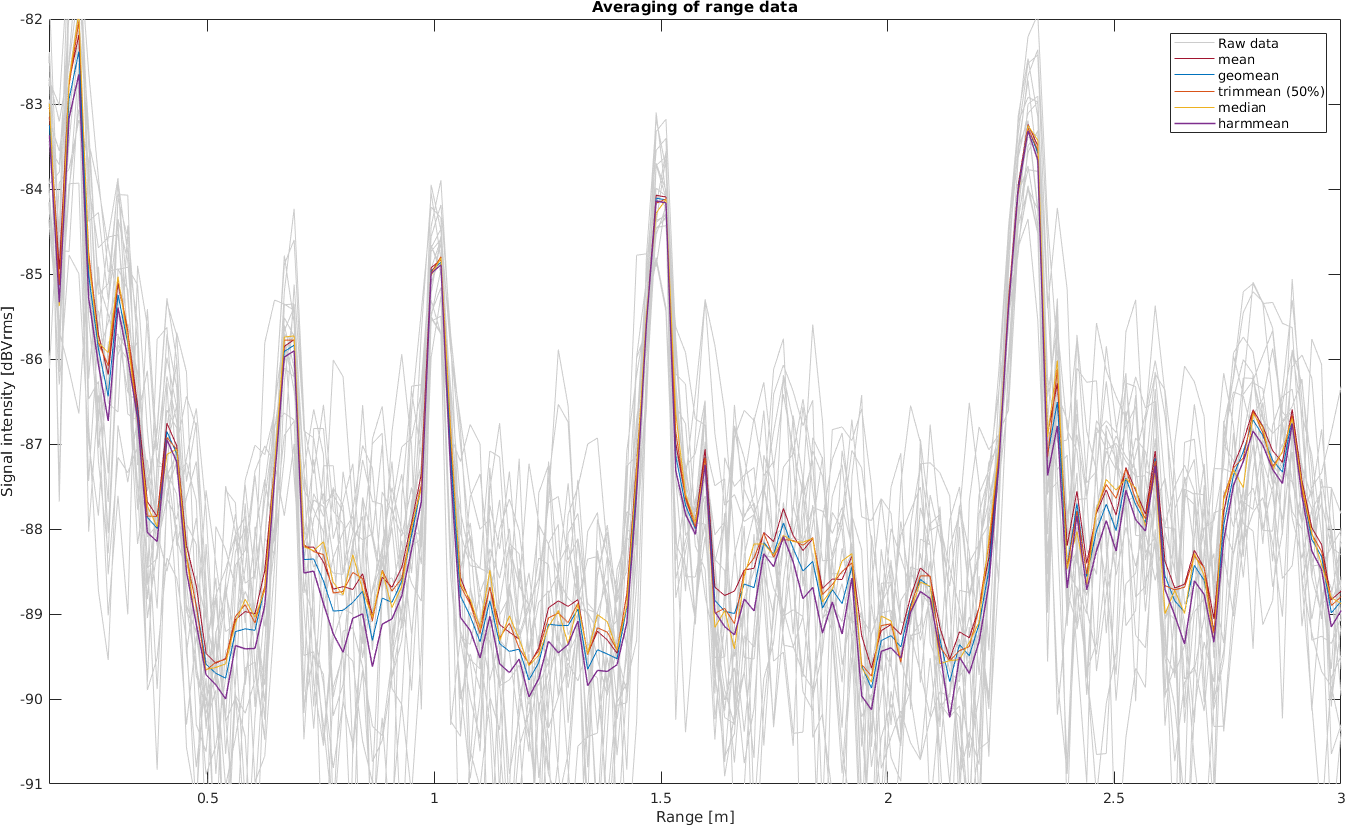
\includegraphics[width=\textwidth]{figures/fig_compare_means}
    \caption{Range profile quality comparison with different averaging functions. Higher peak-to-trough ratio is better.}
    \label{fig:fig_compare_means}
\end{figure}

\Cref{fig:fig_compare_means} shows in gray the raw data of the first 20 range scan lines
from the ``Mancave'' dataset. It then compares different methods of averaging (the three pythagoreans means, a trimmed mean and the median) over these 20 scans. All of them improve the SNR, because the noise is statistically mostly uncorrelated to the signal. Table \cref{tab:mean}
compares the root mean square (RMS) of the difference of each signal to the harmonic mean,
which gives the cleanest signal with the highest SNR.

If the arithmetic mean is defined as
\begin{equation}
        \text{mean}(x_{i=1,2,...,n}) = \frac{1}{n}\sum_{i=1}^n x_i=\frac{x_1+x_2+\cdots+x_n}{n}
\end{equation}

then the RMS of a signal $x_i$ yields
\begin{equation}
    \text{RMS}(x_{i=1,2,...,n}) = \sqrt{\text{mean}(x_i^2)}
\end{equation}

The harmonic mean is defined as
\begin{equation}
    \text{hmean}(x_{i=1,2,...,n})
    = \frac{1}{\text{mean}(x_i^{-1})}
    = \frac{n}{\frac1{x_1} + \frac1{x_2} + \cdots + \frac1{x_n}} = \frac{n}{\sum\limits_{i=1}^n \frac1{x_i}}
\end{equation}

The geometric mean is defined as
\begin{equation}
    \text{gmean}(x_{i=1,2,...,n}) = \left(\prod_{i=1}^n x_i \right)^\frac{1}{n} = \sqrt[n]{x_1 x_2 \cdots x_n}.
\end{equation}
The \SI{50}{\%} trimmed mean is defined as the arithmetic mean of all except
the highest and lowest \(\frac{n}4\) data points, where \(n\) is the
number of data points. The median is defined as the value that lies
between the lower and the upper half of sample values.

The last row denotes the (arithmetic) mean of the value for the raw data $s_{d_{down},d_{cross}}$ of each of the 20 scans,
\begin{equation}
    \text{mean}_{d_{cross}}\Bigl[
        \text{RMS}\Bigl(
            s_{d_{down},d_{cross}} - \text{hmean}_{d_{down}}(s_{d_{down},d_{cross}})
        \Bigr)
    \Bigr]
\end{equation}

{ %\begin{table}[htbp]
    \centering
    \rowcolors{1}{ColorAlternatedRow}{}
    \begin{tabularx}{0.5\textwidth}{XX}
        \hiderowcolors
        \toprule
            Signal & RMS of difference to harmonic mean\tabularnewline
        \midrule
        \endhead
        \showrowcolors
            Harmonic mean & 0\tabularnewline
            Geometric mean & 0.144\tabularnewline
            Arithmetic mean & 0.275\tabularnewline
            \SI{50}{\%} Trim mean & 0.284\tabularnewline
            Median & 0.318\tabularnewline
            Raw data, mean & 1.064\tabularnewline
        \bottomrule
        \caption{Comparison of mean types by RMS}
        \label{tab:mean}
    \end{tabularx}
} %\end{table}

Due to the good signal quality, the implementation uses the harmonic
mean to average the bins. Weighting the average with triangular or
Gauss-shaped weight distribution did not noticeably improve data quality
for any of the averaging methods.

Note that the range signal is not the only signal that needs to be
averaged in a range bin. All other parameters that are part of the range
scan need to be averaged as well. These parameters are mileage at scan
time, robot position and orientation, and robot speed. Sweep time and
down range bins don't change.

\section{Doppler Estimation with the Peak Gradient Algorithm} \label{doppler-estimation-with-the-peak-gradient-algorithm}

The peak gradient algorithm is a way to find Doppler speeds from
consecutive range profiles.

\begin{figure}[htbp]
    \centering
    \begin{subfigure}[t]{\textwidth}
        \def\svgscale{1}
        \input{gfx/fig_svg/explain_peak_gradient_1.pdf_tex}
        \caption{Range profile}
        \label{fig:explain_peak_gradient_1}
    \end{subfigure}\bigskip\\
    \begin{subfigure}[t]{\textwidth}
        \def\svgscale{1}
        \input{gfx/fig_svg/explain_peak_gradient_2.pdf_tex}
        \caption{Range profile in region of interest box}
        \label{fig:explain_peak_gradient_2}
    \end{subfigure}\bigskip\\
    \begin{subfigure}[t]{\textwidth}
        \def\svgscale{1}
        \input{gfx/fig_svg/explain_peak_gradient_3.pdf_tex}
        \caption{Gauss-approximated range profile in region of interest box, with subsample-interpolated peaks}
        \label{fig:explain_peak_gradient_3}
    \end{subfigure}\bigskip
    \caption{Peak detection and subsample peak interpolation to find peak distance between two range profiles}
    \label{fig:fig_explain_peak_gradient}
\end{figure}

In \cref{fig:explain_peak_gradient_1} the scans at radar mileage \SI{0.355}{m} and \SI{0.375}{m} of a scene (``Basement'') are overlaid. At this small cross range difference the range profiles of the two scans are relatively similar. However, as visible in \cref{fig:explain_peak_gradient_2} some peaks from target echoes are shifted, as the distance to the targets changes with the radar moving through the scene. The rate at which the distance to a target changes is its relative speed to the radar, the Doppler speed.

Usually, speed is measured in distance per time. In this case, it
actually makes sense to ignore the scan's time stamps and look at the
cross range (driven mileage) instead. With the Doppler speed as change
of down range (distance to target) per cross range driven, calculations
become time independent and hence radar movement speed independent.

A target's distance from the radar is assumed to be at the range bin of
the corresponding peak in a scan's range profile. When a target's
distance changes the peak will shift, too. This is visible in \cref{fig:explain_peak_gradient_2} and we can read the Doppler speed from the figure. The peak around \SI{0.67}{m} moves \(d_{down,1} = \SI{0.0216}{m}\) closer in range, while the peak
around \SI{0.95}{m} moves \(d_{down,2} = -\SI{0.0216}{m}\) closer (i.e., away).
Combined with the change in cross range,
\(d_{cross} = \SI{0.3752}{m} - \SI{0.3555}{m} = \SI{0.0197}{m}\), we can calculate Doppler
speeds of \(v_{D,1} = \frac{d_{down,1}}{d_{cross}} = \SI{109.55}{\%}\) (of
radar movement speed) and
\(v_{D,2} = \frac{d_{down,2}}{d_{cross}} = -\SI{109.55}{\%}\). If the speeds
were \SI{100}{\%} and -\SI{100}{\%} it would mean that the targets are directly
ahead and directly behind the moving radar. Speeds over \SI{100}{\%} are
however impossible in a static environment where all relative target
motion is caused by the radar movement. The targets are therefore either
dynamic and moving by themselves, or the peak locations that determined
those too-high speeds were not exact. Since we know that there were no
dynamic moving objects in the controlled environment of the scan, the
latter must be the case.

This effect of imprecise target peak localization and Doppler speed
estimation could be overcome by averaging noisy data so that the average
peak distance is close to the actual change in target range. A lot more
scans are necessary for that though, and scan oversampling needs to be
drastically reduced. This would lead to lower SNR, which means that some
peaks with lower echo intensity could not be detected.

With higher downrange resolution, peaks could be localized more
precisely. However, the down range resolution is limited by the
available bandwidth of the radar sensor. In the Omniradar RIC60A, up to
\SI{7}{GHz} are available, which is already extremely high. Its range
resolution \(dR\) is \(\frac{c}{2 BW}\), which is roughly \SI{2.1}{cm}. With
this method, \(dR\) is of course the smallest measurable change of
target range.

The localization of peaks is however not limited by range resolution,
but by range accuracy, which mainly depends on SNR. It is much better
than range resolution with \(\sigma_R = \frac{dR}{\sqrt{SNR}}\). This
can be utilized with subsample peak interpolation.

\subsection{Inter-scan vs Intra-scan Doppler estimation} \label{inter-scan-vs-intra-scan-doppler-estimation}

For correct Doppler estimation it is important to have the exact timing,
or for relative Doppler speed, exact cross range mileage of the range
scans whose peaks are compared in the peak gradient algorithm.

The Omniradar sensor can send multiple consecutive sweeps without any
delay between them. The timing will then be very exact, because the
precise length of one sweep is known. However, the number of sweeps in
such a set of sweeps is limited (transmission of high data volumes will
often fail), so they can't be average to be smoothed through
oversampling and will be noisy. Smaller peaks will then not be detected
reliably. Another problem with this approach is that it will give target
Doppler speeds in change of down range over time, but not the robot
speed-invariant relative Doppler speed in change of down range over
change of cross range.

Inter-scan comparison gives better Doppler estimation, because the data
can be smoothed through oversampling first. Consecutive sweeps can still
be used: They need to be separated into individual scans with timestamps
adjusted to \(t_{msg} + i\cdot t_{sweep}\) (with message timestamp
\(t_{msg}\), consecutive sweep index \(i\) and sweep duration
\(t_{sweep}\)) and cross range mileage interpolated at that timestamp.

\subsection{Subsample peak interpolation}\label{subsample-peak-interpolation}

In subsample peak interpolation a curve is fitted on several supporting
points in the coarse-resolution data. In the case of a single,
non-overlapping radar echo peak, a Gaussian pulse of the form
\[g_i(x) = a_i e^{-b_i ( x - c_i )^2}\] is a good approximation. In
figure \cref{fig:explain_peak_gradient_3}, the data point of the respective peak as well as its left
and right neighbors are fitted with a Gaussian. The fit parameters
\(a\), \(b\) and \(c\) are calculated using Travis
Wiens's crit\_interp\_g function\footnote{\url{https://www.mathworks.com/matlabcentral/fileexchange/24465}}.

As evident by visual inspection, the intensity and location of the
fitted function's maximum are much closer to the real value.

With the same procedure as explained above, we measure peak distance
shifts of \(d_{down,1}=\SI{9.510}{mm}\) and \(d_{down,2}=-\SI{13.52}{mm}\) in figure
\cref{fig:explain_peak_gradient_3} and can hence estimate Doppler speeds of \(v_{D,1}=\SI{48.26}{\%}\) and
\(v_{D,2}=-\SI{68.63}{\%}\) of radar movement speed. These values are a much
more plausible estimation and generally work very well when used to
calculate the reprojection angle in the reprojection method.

\subsection{Peak matching}\label{peak-matching}

Visually it seems clear which peaks belong to each other in consecutive
range scan lines. But for the algorithm this poses a challenge. Range
scan lines usually don't have the same number of peaks because new
targets can appear, old targets can disappear, noise can temporarily
mask out targets peaks and target arcs cross each other. However if the
cross range difference, i.e.~the driven distance between scans, is not
too high, a single target will not change very much in both range and
echo intensity. This allows the detection of peak matches, between which
the Doppler speed will be calculated. The parameters for peak matching
tolerance are therefor allowed intensity change \texttt{ValueSearchArea} and allowed range change \texttt{LocSearchArea}, respectively:
\begin{align}
    \text{\texttt{ValueSearchArea}} &= \frac{\delta I}{\Delta d_{cross}}\\
\intertext{and}
    \text{\texttt{LocSearchArea}} &= \frac{\Delta d_{down}}{\Delta d_{cross}} = v_{D,\max} \stackrel{\text{eq. \ref{eq:geometry_side_B}}}{=} v_R~cos(\alpha)
\end{align}
with intensity change factor $\delta I$ and down range deviation $\Delta d_{down}$ per added cross range mileage $\Delta d_{cross}$.

$\Delta d_{down} / \Delta d_{cross}$ is more easily expressed as Doppler speed \(v_D\) in percent of robot speed \(v_R\). It makes sense to allow \texttt{LocSearchArea}s greater than $1~v_R$ to deal with noise and jitter -- otherwise a target peak closing at roughly $v_R$ would not always be detected and smoothing over cross-range would be worse. The detected $v_D > v_R$ of course need to be clipped to $v_R$ or ignored in reprojection (which is what the current implementation does). Good values are a \texttt{ValueSearchArea} of \SI{5}{cm^{-1}} and a \texttt{LocSearchArea} of \(2~v_R\).

\subsection{Minimum Peak height}\label{minimum-peak-height}
Without countermeasures a lot of noise with low height and low full-width-at-half-maximum will clutter the reprojection map. The easiest way to prevent this is to apply a threshold on the detected peak height that rejects all peaks that do not reach a certain minimum height. It's not easy to specify such a threshold that works for all scans, because the noise floor level strongly depends on the chirp time. \Cref{fig:fig_compare_chirp_times} shows that this persists even when the echo intensity is normalized to intensity 1 at the first range bin before transmit cross talk suppresion (see \cref{transmit-crosstalk-suppression}).

%TODO

\subsection{Transmit crosstalk suppression}\label{transmit-crosstalk-suppression}

At low range, spurious peaks occur. The first one is caused by transmit
antenna crosstalk and is visible as very high intensity echo around
\(d_{down}=0\). After the transmit antenna crosstalk spike there is
another peak around \(d_{down}=\SI{0.25}{m}\) which is consistently visible. It
can be explained with static objects sitting close to the radar,
i.e.~robot parts and the floor below the robot.

These spurious peaks create two problems: (1) automatic color scaling or
height scaling respectively in plots is more difficult, and (2) high
intensity false positives would be visible next to the robot path in the
final map.

Hence these spurious peaks must be ignored during peak detection. This
can be achieved in two ways. The first is to simply replace all data
values under a down range limit \(d_{mute}\) (usually
\(d_{mute}=\SI{0.30}{m}\)) with \(NaN\) values. For the second way, one effect
of range compensation is exploited. As shown in \cref{fig:fig_range_compensation_transmit_spike}, the spike
that previously had its maximum in the first range bin, at
\(d_{down}=0\), now has its maximum in a later range bin. The reason is
that the range compensation factor at \(d_{down}=0\) is \(r(0) = 0\) but
\(r(d_{down}>0) > 0\). As the transmit peak now has a maximum with
neighbors lower than its maximum, \texttt{findpeaks} can find it. Color
scaling can then be made to work correctly by clipping all values higher
than the \emph{second highest} peak. The Peak Gradient Algorithm also
has an optional parameter \texttt{SkipFirstPeak} which, when set to
\(true\), ignores the first peak in each range scan line. This can help
to ignore these echoes.

\begin{figure}[htbp]
    \centering
    \begin{subfigure}[t]{\textwidth}
        \centering
        \def\svgscale{.8}
        \input{gfx/fig_svg/fig_range_compensation_transmit_spike_1.pdf_tex}
        \caption{Linear scale}
        \label{fig:fig_range_compensation_transmit_spike_1}
    \end{subfigure}\bigskip\\
    \begin{subfigure}[t]{\textwidth}
        \centering
        \def\svgscale{.8}
        \input{gfx/fig_svg/fig_range_compensation_transmit_spike_2.pdf_tex}
        \caption{Logarithmic scale (Note that the \(0\) value at \(d_{down}=0\) can not be displayed in log scale.)}
        \label{fig:fig_range_compensation_transmit_spike_2}
    \end{subfigure}
    \caption{Attenuating effect of range compensation on transmit peak in a range profile}
    \label{fig:fig_range_compensation_transmit_spike}
\end{figure}


\subsection{Peaks overlaps at crossing target arcs} \label{peaks-overlaps-at-crossing-target-arcs}
Often there appears a situation where the range cell migration arcs of two targets cross each other. In this case, their peaks can almost always be still detected separately. However peak-associated data like DOA and Doppler speed will superpositioned. Using these in a regular fashion would yield wrong results. An approach that proved to work well in practice is to sort all peaks in a range scan line by ascending value (peak height), then assigning the average over the FWHM of the feature in question to all output down range cells within half the FWHM of the respective peak. Higher peaks are hence treated as more important and overwrite the values of lower peaks. \Cref{fig:overlap} is an example where the overlapping effect is visible.

\begin{figure}[htbp]
    \centering
    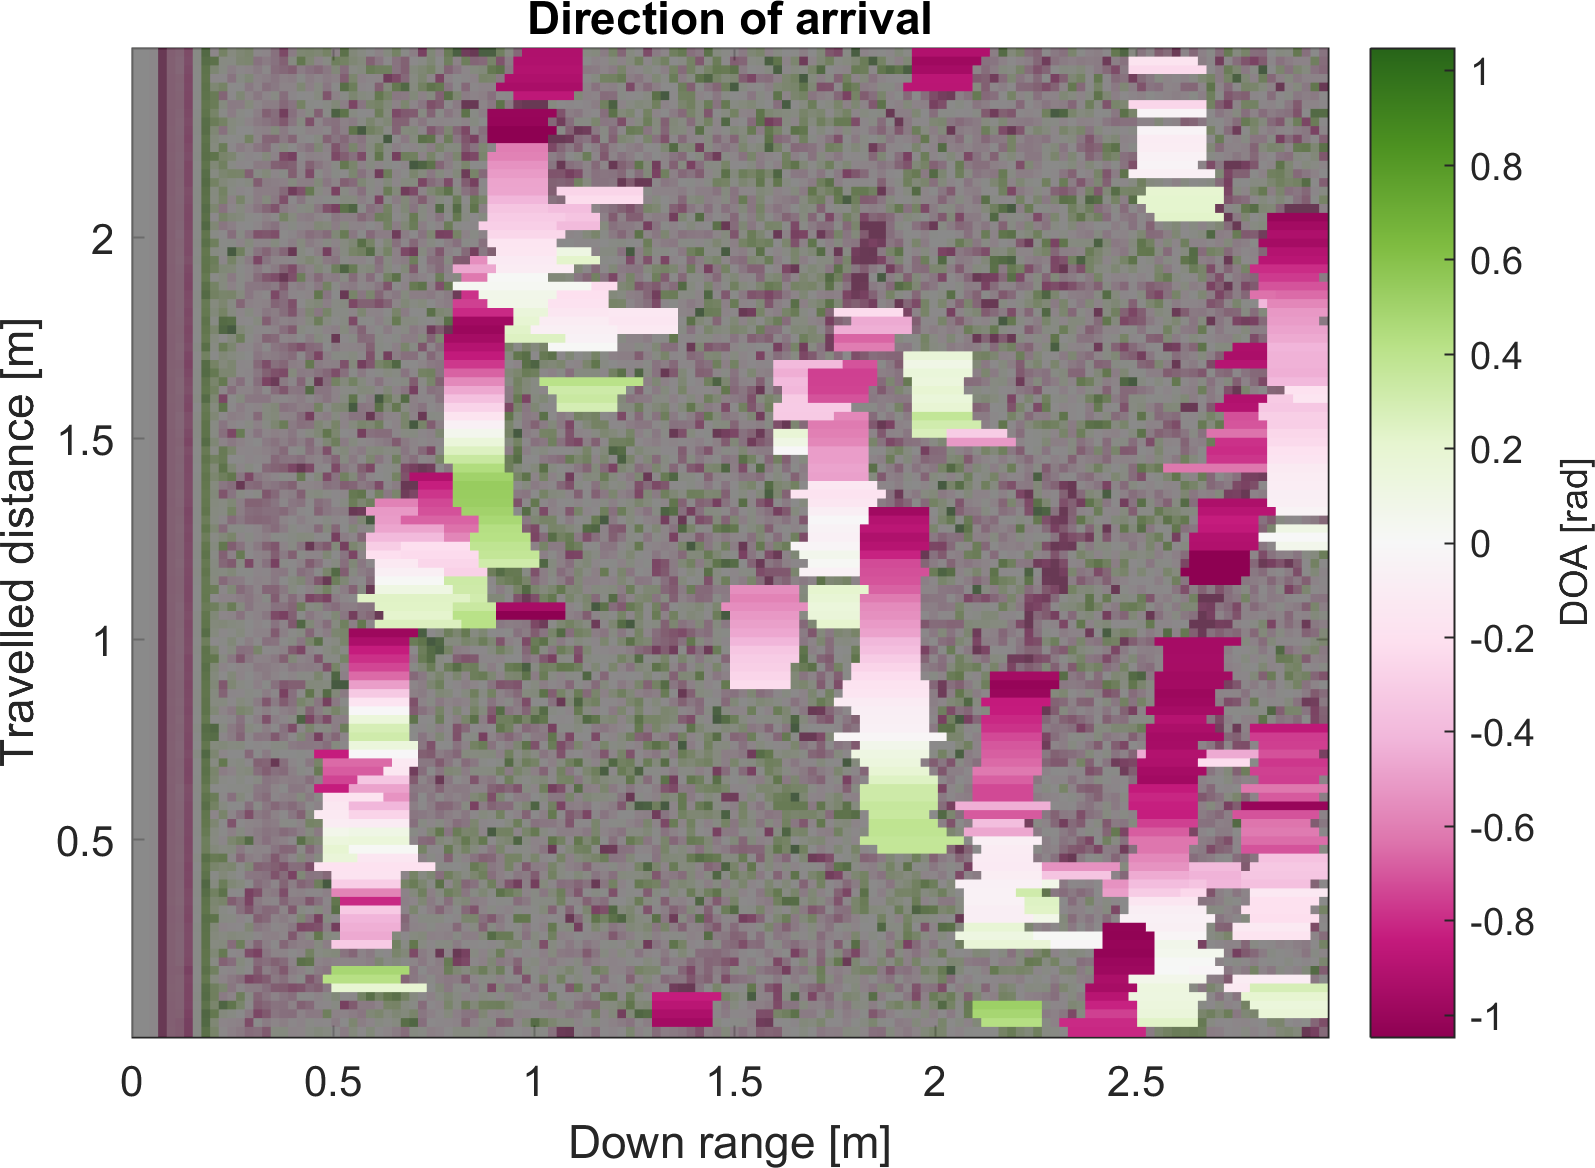
\includegraphics[max width=10cm]{gfx/results/attic_doa.png}
    \caption{DOA of Attic scan. The DOA of higher peak values is applied over the FWHM, superseding the values of lower peak values.}
    \label{fig:overlap}
\end{figure}
TODO annotate in figure where the overlap is

\subsection{Output}\label{output}
In this implementation the resulting size of the reprojection map is known in advance so the map does not need dynamic resizing and can be allocated ahead of time. To make sure everything will fit, the initial size is chosen as \texttt{round[ max(radar\_position) - min(radar\_position) + 2~radar\_max\_range + 2 * 0.2 m ]} in both X and Y dimension.

The \texttt{world\_res\_m} parameter defines the resolution of the gridmap to be created. Larger values (e.g. \SI{10}{cm}) result in coarse homogeneous map, while small values (e.g. \SI{1}{cm}) lead to unmapped area between reprojection lines. The latter is because noise and jitter in Doppler speed estimation cause imprecision in reprojection angles. As explained in \cref{sample-splitting}, the reprojected down range cells of the range scan lines fall into a maximum of four output pixels. With a limited number of reprojections that have slight variations in reprojection angle, this can result in gaps between the output cells. The optimal \texttt{world\_res\_m} is hence somewhere between these extremes, a good value is slightly larger than the down range resolution $dR$, which is around \SI{2.1}{cm} in this implementation.

By saving the output after each processed range scan line and reassembling it, a video of the map buildup can be generated. Otherwise, the map can be trimmed of its empty cells.

For some scans, the \texttt{map} topic is available. In this case, the radar map can be overlaid over the lidar slam gridmap. To achieve this in Matlab, the lidar map is plotted as \texttt{surface} of zero height and an RGB texture that is generated from the values in the gridmap. The radar map is then overlaid as separate surface with an alpha channel of zero opacity for empty reprojection map cells, \SI{70}{\%} opacity for reprojection cells with a normalized value $\ge \SI{70}{\%}$, and linearly mapped opacity between \SIrange{0}{70}{\%} normalized value.

\subsection{Limitations}\label{limitations-1}

Next to the inherent limitations of reprojection mapping (see \cref{limitations}) there are some limitations that arise from the presented implementation.

\subsubsection{Problems with imperfect fit function for subsampling} \label{problems-with-imperfect-fit-function-for-subsampling}
The subsample peak interpolation in \cref{subsample-peak-interpolation} works with a Gaussian fit function. This is a good but not perfect approximation of the real peak shape. The effect only becomes noticeable when the cross-range distance $\Delta d_{cross}$ between (smoothed) range scan lines becomes very small. Interpolated peaks at the center and edges of the down range bins are correctly placed because both the fit function and the true peak shape are symmetric around the true peak. In between those however, peaks are interpolated slightly off because the fit function does not perfectly reflect the true shape of the curve. When examining a peak migrating at a constant speed through the range profile, its subsampled peaks will then lie on an S-shaped path between every (correctly interpolated) cell edge and center. In effect, the Doppler speed estimated with the peak gradient algorithm (see \cref{doppler-estimation-with-the-peak-gradient-algorithm}) will show oscillations around the true Doppler speed. Since wrongly estimated Doppler speeds cause wrong reprojection angles, this causes a radial smearing of targets in the reprojection map.

The effect becomes less noticeable with greater cross-range distances and completely disappears at $\Delta d_{cross} \ge \Delta d_{down}$. Other than increased performance, that is also the reason for choosing a binning approach over a running average for raw data smoothing (see \cref{raw-data-smoothing}).

\subsubsection{Problems with close targets}\label{problems-with-close-targets}

When Doppler speed is measured directly using FMCW, there will be
several Doppler peaks, each representing a different target at the same
range but with individual relative speeds. With the Peak Gradient
Algorithm however, multiple targets at the same range are difficult to
separate. In some cases this is only a temporary problem and is resolved
by the radar moving a little farther so the ranges are separated by more
than the range resolution. Sometimes however some peaks come from
point-like targets that are close together, like a parts of a wall. This
bundle of targets is however not always separated by the same range.
Especially in the case of a wall, the traces of visible points will
cross each other as they slide on the sine arc (see figure). When the
points are close together, only the brightest spots will be seen as
peaks, and the trace of the detected peak matches will describe a
squiggly motion. This causes the estimated Doppler speed to wander
around the common speed. To combat this effect, a higher accumulation
distance can be used during oversampling preprocessing, so the peaks
move together so closely that they actually form a single target.

TODO explanation of "simulation"

\begin{figure}[htbp]
    \centering
    \begin{subfigure}[t]{.5\textwidth}
        \centering
        \def\svgscale{.8}
        \input{gfx/fig_svg/squiggly_doppler_at_wall_1.pdf_tex}
        \caption{Simulation setup}
        \label{fig:squiggly_doppler_at_wall_1}
    \end{subfigure}%
    \hfill%
    \begin{subfigure}[t]{.5\textwidth}
        \centering
        \def\svgscale{.8}
        \input{gfx/fig_svg/squiggly_doppler_at_wall_2.pdf_tex}
        \caption{Simulated input energy}
        \label{fig:squiggly_doppler_at_wall_2}
    \end{subfigure}\bigskip
    \caption{The target echo at the closest range usually has the brightest intensity. This can lead to errors in Doppler speed estimation.}
    \label{fig:squiggly_doppler_at_wall}
\end{figure}

\section{DOA Estimation}\label{doa-implementation}

In geometries as described in \cref{geometry-for-the-general-case}, the next step is to estimate the Direction of Arrival to resolve reprojection angle ambiguities.
As described in \cref{direction-of-arrival}, the Direction of Arrival (DOA) angle can be measured from the phase difference at the receiving antennas of a multistatic radar.

In the case of RIC60A the antenna separation \(d=\SI{1.16}{mm}\) and
wavelength \(\lambda\) is \(\lambda=\frac{c}{\SI{60}{GHz}}=\SI{5.0}{mm}\) (with speed
of light \(c\)).

\Cref{fig:fig_range,fig:fig_phase_shift} show the range profile and phase shift of the
``Basement'' scan. The phase shift is very noisy in the regions without
a target peak in the range profile but exhibits steady values following
a gradient over targets.

\begin{figure}[htbp]
    \centering
    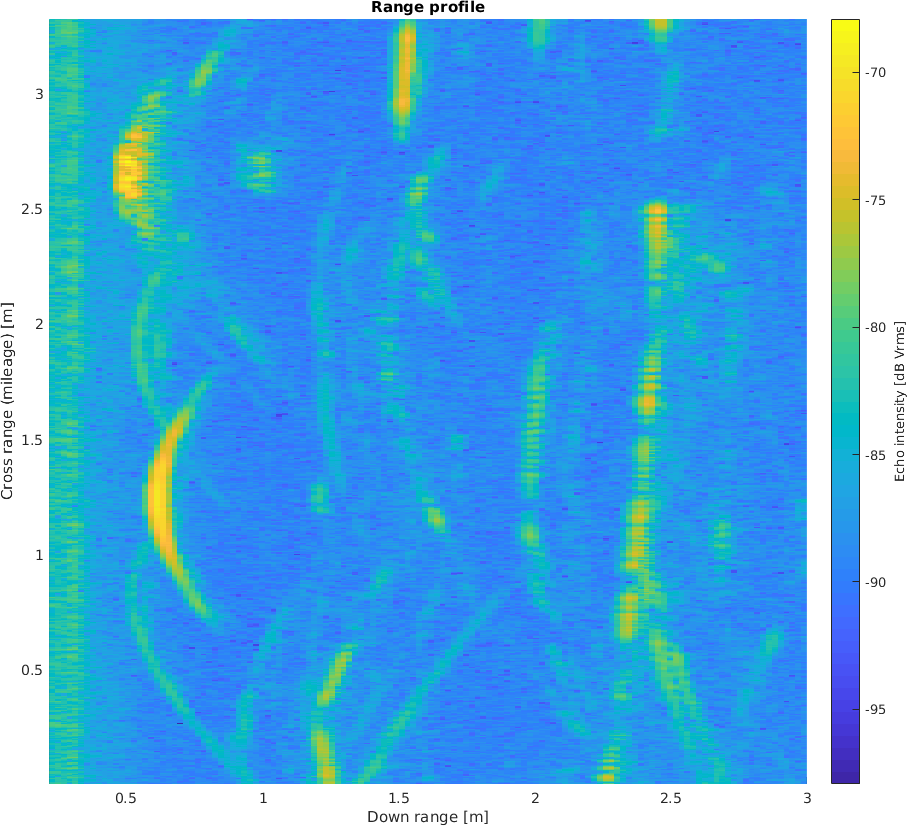
\includegraphics[max height=10cm,max width=10cm]{figures/fig_range}
    \caption{Range profile of Attic scan with color coded echo intensities at cross range over down range}
    \label{fig:fig_range}
\end{figure}

\begin{figure}[htbp]
    \centering
    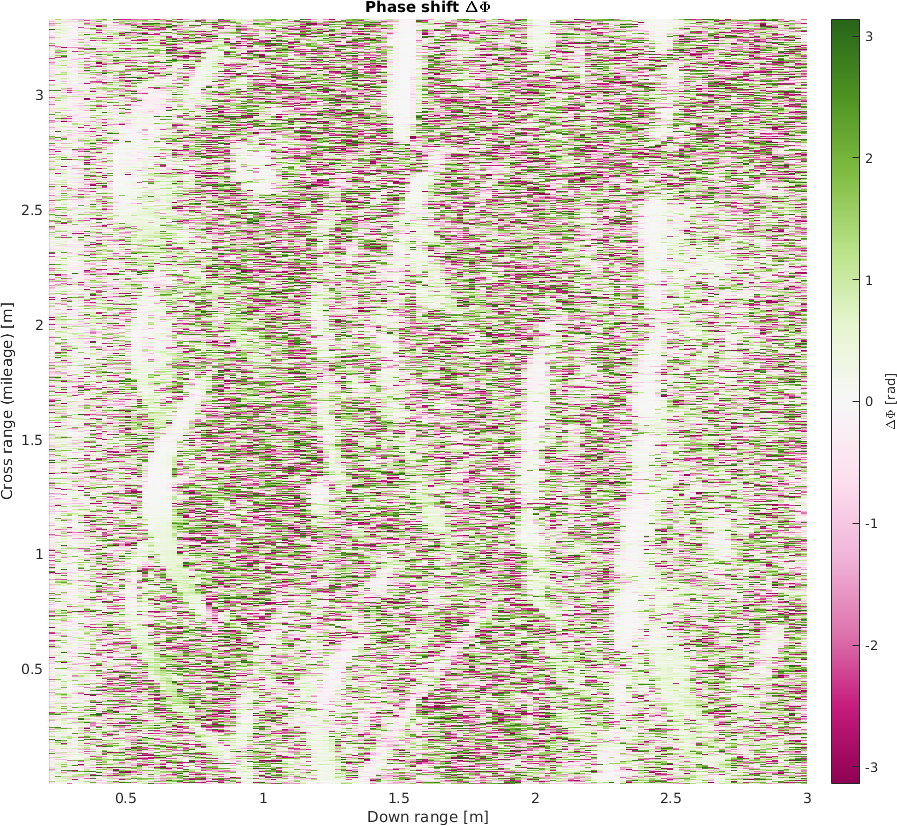
\includegraphics[max height=10cm,max width=10cm]{figures/fig_phase_shift}
    \caption{Phase profile of Attic scan with color coded inter-antenna phase difference at cross range over down range}
    \label{fig:fig_phase_shift}
\end{figure}

Four steps are performed to get a reasonable estimation of direction of
arrival.

\textbf{Peak detection}. In a first step, target peaks in the
range profile are detected. The algorithm records for each peak in each
range scan line its fitted interpolated location, full width at half
maximum, and matching peaks in adjacent lines regarding value and
location.

\textbf{Down range averaging}. In each range scan and at every
detected target peak, the phase shift is averaged over the width of the
respective detected peak. The average is weighted using the Gaussian fit
from subsample peak interpolation.

\textbf{Cross range averaging}. In
every range scan line, each peaks phase shift is averaged over a
configurable accumulation distance in cross range dimension. This is
done by taking the arithmetic mean of all the phase shifts at all
matching peaks (regarding value and down range location) within
accumulation distance in cross range dimension.

\textbf{Cut out}. Noisy
values at non-target peak range bins are masked out.

\textbf{DOA calculation}. In each scan line, each peaks direction of arrival
\(\theta\) is calculated from the smoothed phase shift values, using \cref{eq:doa}.

\Cref{fig:fig_doa} shows the result of these four steps applied on the data of
the ``Basement'' scan. The direction of arrival seems plausible: In this
side-facing scan the robot passed some metal cans. Apparently the radar
sensor was not mounted perfectly orthogonal to the robot's movement
direction (which is not necessary for the reprojection method), but was
slightly off by. This can be seen at the closest points of the target
arcs. At the pericenter the line of sight to a target is orthogonal to
the robot's movement direction, but the DOA value shows to be around \ang{5}
to \ang{10}.

\begin{figure}[htbp]
    \centering
    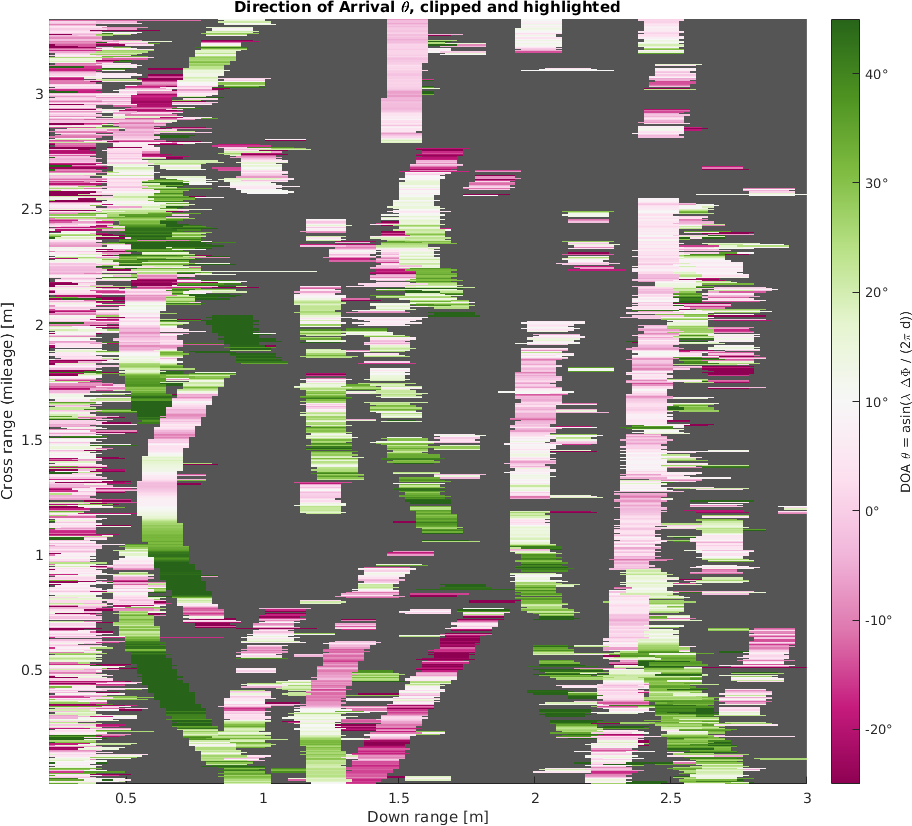
\includegraphics[max height=10cm,max width=10cm]{figures/fig_doa}
    \caption{Direction of arrival estimation for Attic scan}
    \label{fig:fig_doa}
\end{figure}

Note that if the radar sensor is mounted inverted (rotated by \ang{180}), DOA
values have to be multiplied by \(-1\) to keep right and left where they
are.

TODO ric60a doa figure

\section{Reprojection Mapping}\label{reprojection-mapping}

\subsection{Orientation parameters}\label{orientation-parameters}

Before the reprojection can be executed, the physical orientation of the
radar sensor needs to be known to the algorithm. In the implementation,
the two Boolean parameters \texttt{forward\_looking} and
\texttt{mount\_inverted} control the behaviour. If the radar's squint
angle and angle sensitivity are such that the field of view reaches both
sides of the robot path, the \texttt{forward\_looking} parameter needs
to be enabled. This enables the processing of DOA data to find the sign
of every target's reprojection angle i.e.~if it is to the left or right
side of the robot's motion path. If the radar is mounted in an
upside-down configuration the squint angle is not affected, but if the
DOA values are processed they need to be mirrored (multiplication with
\(-1\)) because the left and right antennas are switched. Otherwise,
targets will be projected to the wrong side of the robot's path.

\subsection{Projection direction}\label{projection-direction}

The radar reprojection can be executed as forward or backward mapping.
The proof of concept implementation has an optional parameter
\texttt{ProjectionMethod} to switch between forward and backward
mapping.

\subsubsection{Backward mapping}\label{backward-mapping}

If backward mapping is enabled, the reprojection algorithm still
operates range scan line based, but iterates over each pixel in the map.
While this is computationally much more intensive, it allows to add
negative information by reducing the map's value at pixels that are
known to not contain a target because the range scan line does not
feature a peak at that range.

\begin{verbatim}
foreach range_scan_line in range_scan_lines
  foreach pixel in map
    pixel_angle = robot.get_angle_to(pixel)
    distance = robot.get_distance_to(pixel)
    if distance < max_range && pixel_angle in field_of_view_range
      range_bin = range_scan_line.interpolate_at(distance)
      if range_bin.has_peak
        peak_angle = range_bin.peak.doppler.to_angle
        if peak_angle == pixel_angle
          map.at(pixel).add(range_bin.value)
      else
        map.at(pixel).reduce_value
\end{verbatim}

\subsubsection{Forward mapping}\label{forward-mapping}

In forward mapping, the reprojection algorithm iterates over each range
bin in each range scan line. Detected peaks are cut out and reprojected
to a position on the map which is calculated from relative Doppler
speed, range, and robot position. The projection target coordinates
don't usually fall exactly on the map grid points. The implementation
uses sample splitting to distribute a value over the nearest pixels in
this case.

\begin{verbatim}
foreach range_scan_line in range_scan_lines
  foreach peak in range_scan_line
    foreach range_bin in peak
      target_coords = get_coords(robot.position, range_bin.range, peak.doppler)
      weights, neighborhood = split_sample(target_coords)
      map.at(neighborhood).add(weights, range_bin.value)
\end{verbatim}

\subsection{Sample splitting}\label{sample-splitting}

To avoid aliasing when projecting a pixel in the forward projection
direction, the sample is split over the four closest map pixels. The
split is weighted with the distance of the target coordinates to the
closest pixel centers.

If the target coordinate is \(p_{target}=(x_t, y_t)\), then the
horizontal and vertical distributions \(\nu_h\) and \(\nu_v\),
respectively, are \[
\nu_h = \frac{x_t - \lfloor x_t \rfloor}{\lceil x_t \rceil - \lfloor x_t \rfloor} \\
\nu_v = \frac{y_t - \lfloor y_t \rfloor}{\lceil y_t \rceil - \lfloor y_t \rfloor}
\]

The pixel weights \(p_{x,y}\) are then \[
p_{\lfloor x_t \rfloor, \lfloor y_t \rfloor} = \nu_v \nu_h\\
p_{\lfloor x_t \rfloor, \lceil y_t \rceil} = \nu_v (1 - \nu_h)\\
p_{\lceil x_t \rceil, \lfloor y_t \rfloor} =  (1 - \nu_v) \nu_h\\
p_{\lceil x_t \rceil, \lceil y_t \rceil} = (1 - \nu_v) (1 - \nu_h)
\] , such that \[
\sum\limits_{
x \in \{\lceil x_t \rceil, \lfloor x_t \rfloor\}\\
y \in \{\lceil y_t \rceil, \lfloor y_t \rfloor\}
} p_{x,y} = 1
\]

In the special case where $y\_t = \lceil y\_t \rceil = \lfloor y\_t\rfloor$ there are only two instead of the four neighboring pixels. Their weights \(p_{x,y}\) are \[
p_{\lfloor x_t \rfloor, y_t} = \nu_h\\
p_{\lceil x_t \rceil, y_t} = (1 - \nu_h)
\] The same applies when $x\_t = \lceil x\_t \rceil = \lfloor x\_t\rfloor$: \[
p_{x_t, \lfloor y_t \rfloor} = \nu_v\\
p_{x_t, \lceil y_t \rceil} = (1 - \nu_v)
\] And lastly, if
(\(y_t = \lceil y_t \rceil = \lfloor y_t \rfloor ) \land (x_t = \lceil x_t \rceil = \lfloor x_t \rfloor )\),
then \(p_{x_t, y_t} = 1\)

\begin{figure}[htbp]
    \centering
    \def\svgwidth{10cm}
    \input{gfx/diagrams/sample_splitting.pdf_tex}
    \caption{Illustration of a pixel value (white circle) being distributed over the four nearest grid neighbors. The shade of the neighbor's area indicates the individual distribution weight.}
    \label{fig:Sample_splitting}
\end{figure}

\subsection{Range compensation}\label{range-compensation}

As evident from the classical radar \cref{eq:radarclassical}, echo intensity decreases with
the fourth power of distance. This has the effect that reprojected
targets appear brighter when they are mapped from close distance; but
most importantly, when targets are detected from a far distance, mapped
intensities are decreased due to the map's averaging.

This attenuation can be compensated with a range-based compensation
factor \(f_r\) with \[f_r(d_{down}) = {
\left(
c_a + (
\frac{{d_{down}}{c_b}}
+ c_c)^{-4}
\right) ^ {-1}
}\]


\Cref{fig:fig_range_compensation} shows the range profile of the ``Torture Chamber'' scan
both as oversampled raw values (top subplot) and with range compensation
enabled (bottom subplot). The middle subplot details the range scan line
at one cross range highlighted by the red lines. Inspecting this detail
graph reveals that both target peaks and noise floor are lowered in the
near range, while the noise floor stays constant in the far range. This
helps to keep a target's intensity at at least similar values over all
ranges in the map.

TODO split in subfigures, adjust refs
\begin{figure}[htbp]
    \centering
    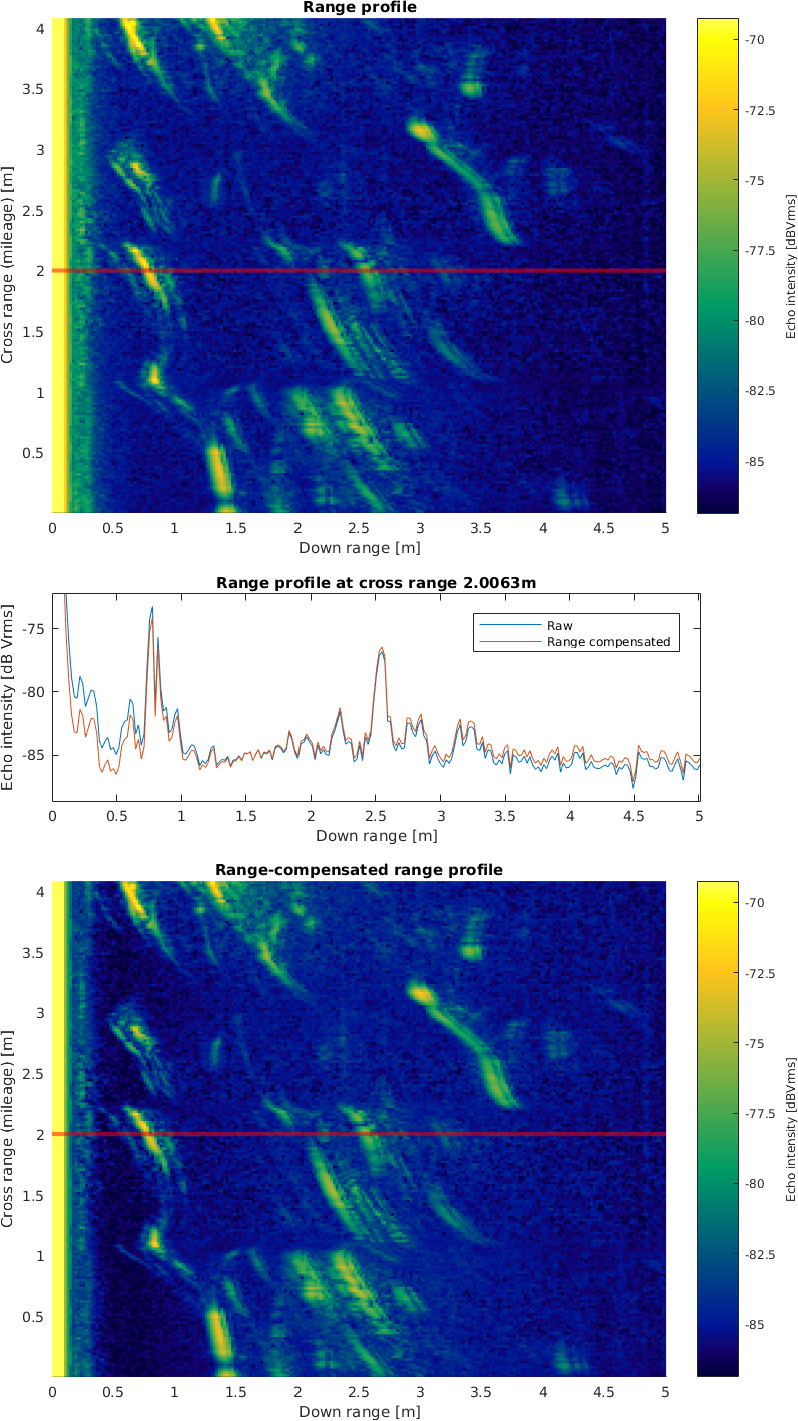
\includegraphics[max width=10cm]{figures/fig_range_compensation}
    \caption{Range compensation}
    \label{fig:fig_range_compensation}
\end{figure}

\subsection{Angle sensitivity compensation}\label{angle-sensitivity-compensation}

The intensity of a target peak depends on its angle with respect to the
antenna. The angle is unknown before the Doppler speed is estimated, so
the knowledge about echo attenuation caused by antenna angle sensitivity
can not be used to improve peak detection. But the echo intensity
influences how a target is represented on the reprojection map. Since
the map averages all reprojections to any given point a low intensity
echo will reduce the visibility of a target on the map. This can however
be compensated by multiplying detected target peak heights with a factor
that is based on the angle the target is believed to be seen under.

The angle compensation factor curve was found by experiment. A strong
point target (a retroreflector) was placed at a known range away from
the robot. The robot was then made to rotate around itself, such that
the target comes into view and leaves again. Meanwhile, the radar scans,
together with robot odometry were recorded.

The radar was not mounted over the center of rotation of the robot. This
way, the radar did describe a circular path whose mileage can be
calculated. The angle compensation measurement can hence be visualized
in figure \cref{fig:fig_range_compensation} in the usual range profile with echo intensities over
cross versus down range. The range of the retroreflector varies with
twice the distance of the radar to the robot's rotation center, but only
the orientation is interesting - the range can just be summed up over
the range bins the target is visible in (in this case,
\SIrange{0.45}{0.85}{m}).

In figure \cref{fig:fig_range_compensation}, the same range scan lines are sorted by robot
orientation during the scan. After the explained summing in down range
dimension the intensity (absolute value of complex signal) data of both
antennas is binned separately over 60 orientations from \(-\pi\) to
\(\pi\).

The manufacturer later provided angle sensitivity measurements of the
IC's manufacturing batch. The measurements show that the
experimental approach produced valid results.

The compensation factor \(f_a\) for each angle is finally composed using
the formula

\[m = \max \left( \max (s_{Rx1}), \max (s_{Rx2}) \right)\] \[
f_a = \frac{1}{2}
  \left(
    \frac{m}{ s_{Rx1} } +
    \frac{m}{ s_{Rx2} }
  \right)
\]

Multiplicating a peak which is to be reprojected at angle \(\alpha\)
with angle compensation factor \(f_a(\alpha)\) results in a peak height
that is independent of observation angle.

\begin{figure}[htbp]
    \centering
    \begin{subfigure}{\textwidth}
        \centering
        \def\svgscale{0.8} \small
        \input{gfx/fig_svg/angle_compensation_1.pdf_tex}
        \caption{Range profile, as recorded}
        \bigskip
    \end{subfigure}
    \begin{subfigure}{\textwidth}
        \centering
        \def\svgscale{0.8} \small
        \input{gfx/fig_svg/angle_compensation_2.pdf_tex}
        \caption{Range profile, sorted by robot orientation}
        \bigskip
    \end{subfigure}
    \begin{subfigure}{\textwidth}
        \centering
        \def\svgscale{0.8} \small
        \input{gfx/fig_svg/angle_compensation_3.pdf_tex}
        \caption{Echo intensity between \SI{0.4}{m} and \SI{0.8}{m} down range, and compensation factor normalizing intensity}
        \bigskip
    \end{subfigure}
    \caption{Angle compensation factor}
    \label{fig:fig_angle_compensation}
\end{figure}

\subsection{Angle compensation window}\label{angle-compensation-window}

Detected peaks are not in a single range bin, but form a curve over
several range bins. Multiplicating each of these range bin's values with
the same \(f_a\) does work, but leaves hard edges. It is better to
multiplicate the peak with a window function with height \(f_a\). The
implementation the window \(w\):
\[
w(x,f_a) = 1 + (f_a - 1) ~e ^ { -\frac{ \left( {x - p_x} \right) ^ 2 } {p_w} }
\] where \(p_x\) is the peaks subsample-interpolated peak location in
down range space and
\[
p_w = \cfrac{
\left( \frac{fwhm}{4}  \right) ^2
}{
4 ln(2)}
\]
is
the peaks width, where \(fwhm\) is the full width at half maximum as
found by the subsample-interpolated peak fit.

\Cref{fig:fig_angle_compensation_comparison} show a glass wall in the ``Racetrack'' scan. In \cref{fig:fig_angle_compensation_comparison_1}, only range compensation is applied. In \cref{fig:fig_angle_compensation_comparison_2},
angle compensation is switched on. In \cref{fig:fig_angle_compensation_comparison_3}, both angle
compensation and angle compensation windowing are switched on. The
figure shows how angle compensation helps to keep the echo intensity of
a mapped object at the same level, regardless of the angle at which it
is seen by the radar.

\begin{figure}[htbp]
    \centering
    \begin{subfigure}{\textwidth}
        \centering
        \def\svgscale{0.8} \small
        \input{gfx/fig_svg/angle_compensation_comparison_1.pdf_tex}
        \caption{Reprojected energy, without angle compensation}
        \label{fig:fig_angle_compensation_comparison_1}
        \bigskip
    \end{subfigure}
    \begin{subfigure}{\textwidth}
        \centering
        \def\svgscale{0.8} \small
        \input{gfx/fig_svg/angle_compensation_comparison_2.pdf_tex}
        \caption{Reprojected energy, with angle compensation}
        \label{fig:fig_angle_compensation_comparison_2}
        \bigskip
    \end{subfigure}
    \begin{subfigure}{\textwidth}
        \centering
        \def\svgscale{0.8} \small
        \input{gfx/fig_svg/angle_compensation_comparison_3.pdf_tex}
        \caption{Reprojected energy, with windowed angle compensation}
        \label{fig:fig_angle_compensation_comparison_3}
        \bigskip
    \end{subfigure}
    \caption{Effect of angle compensation and windowed angle compensation}
    \label{fig:fig_angle_compensation_comparison}
\end{figure}
